%-------------------------------------------------------------------------------
%                            BAB II
%               TINJAUAN PUSTAKA DAN DASAR TEORI
%-------------------------------------------------------------------------------
%\fancyhf{}
% \fancyfoot[C]{\thepage}
\chapter{TINJAUAN KEPUSTAKAAN}

\section{Pengertian Data}
Data merupakan kumpulan fakta, angka, hasil pengukuran, atau deskripsi suatu fenomena yang dikumpulkan untuk dijadikan dasar dalam analisis dan pengambilan keputusan \citep{akerkar2016}. Dalam analisis deret waktu iklim, data terdiri atas dua komponen utama, yaitu \textit{signal} (pola atau karakteristik sebenarnya) dan \textit{noise} (gangguan acak dari kesalahan pengukuran, kondisi lingkungan, atau variasi sensor). Keberadaan \textit{noise} dapat mengurangi representativitas informasi jika tidak ditangani pada tahap awal pengolahan data.

Sebelum memasuki tahap analisis lanjutan, data perlu menjalani \textit{plausibility check} untuk mengevaluasi kelengkapan, konsistensi, dan representativitas data \citep{berthold2020}. Secara umum, pengolahan data diawali dengan \textit{data cleaning} untuk memperbaiki kualitas data, dilanjutkan dengan \textit{smoothing} untuk mengurangi \textit{noise} tanpa menghilangkan pola utama, serta \textit{feature selection} untuk memilih variabel paling relevan.
\section{Data BMKG}
Badan Meteorologi, Klimatologi, dan Geofisika (BMKG) adalah Lembaga Pemerintah Non-Kementerian (LPNK) yang bertanggung jawab dalam penyediaan informasi meteorologi, klimatologi, kualitas udara, dan geofisika di Indonesia \citep{sujalu2020}. BMKG melakukan pengamatan dan pengelolaan data iklim melalui sebaran jaringan stasiun pengamatan di berbagai wilayah guna mendukung kebutuhan pemantauan cuaca, analisis iklim, dan mitigasi bencana sesuai dengan UU Nomor 31 Tahun 2009 \citep{saragih2024}.

Dalam penelitian ini, data BMKG yang digunakan berasal dari Stasiun Klimatologi Aceh Besar dan berbentuk data \textit{time-series} harian yang memuat berbagai parameter iklim hasil pengamatan stasiun dalam format harian. Namun data BMKG memiliki keterbatasan dalam hal fleksibilitas, karena data hanya tersedia dalam format Excel dan tidak menyediakan API \textit{public}.

\section{Data NASA POWER}
NASA \textit{Prediction of Worldwide Energy Resources} (POWER) merupakan layanan data iklim dan meteorologi global yang dikembangkan oleh \textit{National Aeronautics and Space Administration} (NASA). NASA POWER menyediakan berbagai parameter iklim dari observasi satelit dan data \textit{reanalysis}, diantaranya suhu udara, kelembaban, curah hujan, radiasi matahari, dan kecepatan angin, yang banyak digunakan untuk mendukung penelitian iklim, pertanian, serta pengelolaan sumber daya alam \citep{rodrigues2021}. NASA POWER menyediakan akses data melalui API sehingga memudahkan proses akuisisi secara konsisten \citep{sparks2018}.

\textit{Dataset} NASA POWER yang digunakan berbentuk data \textit{time-series} harian yang memuat berbagai parameter iklim hasil estimasi satelit. Berbeda dengan data observasi lapangan BMKG, NASA POWER memiliki ketersediaan lebih lengkap, namun berpotensi mengandung \textit{noise} dan ketidakpastian akibat proses estimasi. Diperlukan juga tahapan \textit{preprocessing} dan \textit{smoothing} untuk mengurangi fluktuasi yang tidak representatif serta mempertahankan pola dan tren iklim.

\section{Pemrosesan Data Iklim}
Pemrosesan data iklim merupakan rangkaian tahapan untuk mengubah data mentah dari sumber observasi menjadi data yang konsisten, bersih, dan siap digunakan untuk analisis \citep{alsalehy2025}. Dalam literatur meteorologi, alur pemrosesan data mencakup penyeragaman format data, pemeriksaan kualitas, deteksi anomali, imputasi nilai hilang, penghalusan data (\textit{smoothing}), serta evaluasi statistik akhir.

Pemrosesan data iklim terdiri atas enam tahapan utama yang disajikan pada pada Tabel \ref{tab:tahapan_preprocessing} berikut:
\begin{table}[H]
\centering
\caption{Tahapan Pemrosesan Data Iklim}
\label{tab:tahapan_preprocessing}
\small
\begin{tabular}{|p{3.5cm}|p{5cm}|p{4cm}|}
\hline
\textbf{Tahapan} & \textbf{Tujuan} & \textbf{Penjelasan} \\
\hline
Validasi awal & Menyamakan struktur dan format data & Standarisasi format waktu, satuan, dan penghapusan duplikasi \\
\hline
Kontrol kualitas & Mendeteksi nilai tidak wajar & Uji batas fisik dan konsistensi temporal \\
\hline
Deteksi \textit{outlier} & Memisahkan anomali dari nilai ekstrem valid & IQR, Z-score, dan pengecekan domain nilai \\
\hline
Imputasi nilai hilang & Mengisi data hilang & Interpolasi linear \\
\hline
\textit{Smoothing} & Mengurangi fluktuasi acak & \textit{Cubic spline}, \textit{adaptive exponential smoothing}, dan \textit{moving average} \\
\hline
Evaluasi kualitas & Menilai hasil pemrosesan & GCV dan \textit{trend preservation} \\
\hline
\end{tabular}
\end{table}

Meskipun mengikuti alur yang sama, penerapan pemrosesan pada data BMKG dan NASA POWER memiliki perbedaan signifikan berdasarkan karakteristik masing-masing. Data BMKG merupakan data observasi lapangan sehingga cenderung mengandung nilai hilang dan inkonsistensi, sehingga fokus utama pemrosesan adalah imputasi dan validasi ketat. Namun, data NASA POWER merupakan hasil reanalisis berbasis satelit secara temporal lebih lengkap namun mengandung \textit{noise}, sehingga pemrosesan lebih difokuskan pada pengurangan \textit{noise} melalui metode \textit{smoothing} agar pola dan tren iklim tetap dapat direpresentasikan tanpa distorsi.

\section{Metode \textit{Smoothing}}
\textit{Smoothing} merupakan salah satu tahapan dalam proses \textit{preprocessing} data yang bertujuan untuk mengurangi pengaruh \textit{noise} tanpa menghilangkan pola utama (\textit{signal}) pada data \textit{time-series}. Proses ini menghasilkan data yang lebih halus sehingga karakteristik tren dan pola musiman menjadi lebih mudah dianalisis serta lebih representatif untuk digunakan pada tahap pemodelan maupun \textit{forecasting} \citep{castillo2022}.

Berbagai metode \textit{smoothing} telah dikembangkan sesuai dengan karakteristik data yang dihadapi. Penelitian ini membahas beberapa pendekatan dasar, yaitu \textit{Moving Average}, \textit{Exponential Smoothing}, \textit{Cubic Spline}, serta \textit{Adaptive Exponential Smoothing}. Masing-masing metode memiliki prinsip kerja yang berbeda dalam mengurangi \textit{noise} dan mempertahankan informasi penting pada data.

\subsection{\textit{Single exponential smoothing}}
\textit{Single exponential smoothing} merupakan metode \textit{forecasting} untuk data \textit{time-series} yang memiliki pola relatif stabil tanpa tren maupun musiman. Metode ini menghasilkan nilai prediksi dengan memberikan bobot yang lebih besar pada observasi terbaru dan bobot yang semakin kecil secara eksponensial terhadap observasi sebelumnya. Tingkat pengaruh data terbaru dikendalikan oleh parameter pemulusan ($\alpha$), sehingga pemilihan nilai $\alpha$ menjadi faktor penting dalam menentukan kualitas hasil peramalan. SES banyak digunakan untuk peramalan jangka pendek karena sederhana, efisien, dan mampu merespons perubahan data secara bertahap \citep{ostertagova2012}.

\subsection{\textit{Double exponential smoothing}}
\textit{Double exponential smoothing} merupakan pengembangan dari \textit{single exponential smoothing} untuk mengatasi data yang memiliki kecenderungan tren. Selain melakukan pemulusan terhadap nilai observasi, metode ini juga mengestimasi komponen tren sehingga mampu menghasilkan prediksi yang lebih baik pada data yang menunjukkan kenaikan atau penurunan secara konsisten. Oleh karena itu, DES lebih sesuai digunakan pada deret waktu yang memiliki pola tren namun belum menunjukkan pola musiman \citep{andriani2022}.

\subsection{\textit{Triple exponential smoothing}}
\textit{Triple Exponential Smoothing} atau metode Holt-Winters merupakan pengembangan lebih lanjut dari metode Holt dengan menambahkan komponen musiman (\textit{seasonality}) ke dalam proses peramalan. Metode ini melakukan pemulusan terhadap tiga komponen utama, yaitu level, tren, dan musiman, sehingga mampu memodelkan data \textit{time-series} yang memiliki pola musiman berulang. Karena mempertimbangkan ketiga komponen tersebut secara bersamaan, Holt-Winters banyak digunakan pada data yang menunjukkan tren sekaligus pola musiman, termasuk berbagai data klimatologi dan meteorologi \citep{andriani2022}.

Dengan mempertimbangkan karakteristik data, penelitian ini menggunakan metode Holt-Winters pada tahap \textit{forecasting} yang dilakukan oleh anggota tim lain, sedangkan penelitian ini berfokus pada tahapan \textit{preprocessing} dan \textit{smoothing} data sebelum proses peramalan dilakukan.
\subsection{Basis \textit{Cubic spline}}
\textit{Cubic Spline} merupakan salah satu metode \textit{smoothing} nonparametrik yang membentuk kurva halus menggunakan serangkaian fungsi polinomial orde tiga (\textit{cubic polynomial}) pada setiap interval data. Setiap segmen polinomial dihubungkan pada titik-titik tertentu (\textit{knots}) sehingga kurva yang dihasilkan tetap kontinu, baik pada fungsi maupun turunan pertamanya. Karakteristik tersebut memungkinkan \textit{Cubic Spline} mengikuti perubahan pola data secara halus tanpa menghasilkan perubahan yang bersifat tiba-tiba.

Berbeda dengan metode rata-rata bergerak maupun \textit{exponential smoothing} yang melakukan pemulusan berdasarkan bobot observasi, \textit{Cubic Spline} membangun suatu fungsi kontinu yang menyeimbangkan antara kedekatan terhadap data asli dan tingkat kehalusan kurva. Secara matematis, \textit{cubic smoothing spline} diperoleh melalui proses optimasi terhadap \textit{penalized weighted mean squared error}, sehingga kurva yang dihasilkan tidak hanya mengikuti data observasi, tetapi juga mengurangi fluktuasi yang disebabkan oleh \textit{noise} \citep{degiosa2024}.

Karena mampu mempertahankan bentuk kurva dan tren utama dengan baik, metode \textit{Cubic Spline} banyak diterapkan dalam analisis data atmosfer, klimatologi, serta berbagai data \textit{time-series} yang memiliki fluktuasi alami \citep{wust2017}.

\subsection{\textit{Exponentially Weighted Moving Average (EWMA)}}

\textit{Exponentially Weighted Moving Average} (EWMA) merupakan metode \textit{smoothing} yang memberikan bobot lebih besar pada observasi terbaru dan bobot yang semakin kecil secara eksponensial terhadap observasi yang lebih lama. Berbeda dengan \textit{Moving Average} yang memberikan bobot sama pada setiap data dalam suatu jendela pengamatan, EWMA menggunakan parameter pemulusan ($\alpha$) untuk mengatur pengaruh data terbaru terhadap hasil \textit{smoothing}. Nilai $\alpha$ yang besar membuat metode lebih responsif terhadap perubahan data, sedangkan nilai yang kecil menghasilkan kurva yang lebih halus karena lebih mempertimbangkan informasi historis. Karakteristik tersebut menjadikan EWMA banyak digunakan pada analisis \textit{time-series} untuk mengurangi fluktuasi acak tanpa menghilangkan pola utama data \citep{javed2024}.

\subsection{\textit{Adaptive exponential smoothing}}
\textit{Adaptive Exponential Smoothing} merupakan pengembangan dari \textit{Exponentially Weighted Moving Average} (EWMA) yang menggunakan parameter pemulusan ($\alpha$) secara adaptif sesuai karakteristik data \citep{andrasto2023}. Berbeda dengan EWMA konvensional yang menggunakan nilai $\alpha$ tetap, metode ini menyesuaikan nilai $\alpha$ berdasarkan tingkat volatilitas lokal pada deret waktu.

Pada kondisi data yang relatif stabil, nilai $\alpha$ dibuat lebih kecil sehingga proses \textit{smoothing} menjadi lebih kuat dan mampu mengurangi fluktuasi acak. Sebaliknya, ketika data mengalami volatilitas tinggi, nilai $\alpha$ diperbesar agar perubahan yang signifikan tetap dapat dipertahankan. Dengan mekanisme tersebut, \textit{Adaptive Exponential Smoothing} mampu menghasilkan proses pemulusan yang lebih responsif terhadap dinamika data tanpa menghilangkan pola utama pada \textit{time-series}.

\section{Evaluasi Kualitas Data}
Setelah melalui proses \textit{preprocessing}, diperlukan evaluasi untuk memastikan bahwa data hasil pemrosesan memiliki kualitas yang baik dan tetap mempertahankan karakteristik utama dari data asli. Dalam penelitian ini, evaluasi dilakukan menggunakan dua metrik, yaitu \textit{Generalized Cross-Validation} (GCV) untuk menilai kualitas hasil \textit{smoothing}, serta \textit{trend preservation} untuk mengukur sejauh mana pola tren pada data tetap terjaga setelah proses \textit{preprocessing}. Kedua metrik tersebut digunakan sebagai dasar dalam menilai kelayakan data sebelum digunakan pada tahap analisis dan \textit{forecasting}.

\subsection{\textit{Generalized Cross-Validation (GCV)}}
Parameter $\lambda$ berperan mengontrol tingkat kehalusan kurva, di mana nilai lebih besar menghasilkan kurva lebih halus namun berpotensi mengurangi sensitivitas terhadap variasi lokal data \citep{wust2017}. Pemilihan parameter optimal dilakukan menggunakan \textit{Generalized Cross-Validation} (GCV), yang merupakan metode estimasi parameter pada \textit{smoothing spline} nonparametrik. GCV memiliki keunggulan karena tidak bergantung pada transformasi ortogonal dan bersifat invarian terhadap rotasi data. Secara matematis, GCV didefinisikan sebagai:
\begin{equation}
    \text{GCV}(\lambda) = \frac{\frac{1}{n} \sum_{i=1}^{n} \left( y_i - \hat{y}_i \right)^2}{\left( 1 - \frac{\text{tr}(\mathbf{S}_\lambda)}{n} \right)^2}
\end{equation}

dengan:
\begin{itemize}
    \item $n$ = jumlah observasi,
    \item $y_i$ = nilai observasi ke-$i$,
    \item $\hat{y}_i$ = hasil estimasi \textit{smoothing},
    \item $\text{tr}(\mathbf{S}_\lambda)$ = derajat kebebasan efektif model.
\end{itemize}

Parameter $\lambda$ optimal diperoleh dari nilai GCV minimum. Penelitian \cite{adams2023} menunjukkan bahwa GCV merupakan pendekatan yang efektif dalam pemilihan parameter pada data, meskipun pada kondisi tertentu dengan autokorelasi tinggi diperlukan evaluasi tambahan terhadap stabilitas estimasi.
\subsection{\textit{Trend preservation}}
\textit{Trend preservation} merujuk pada tingkat kemampuan metode \textit{smoothing} dalam mempertahankan arah dan pola perubahan jangka panjang dari data asli setelah proses pemrosesan. Dalam analisis \textit{time-series}, aspek ini menjadi penting karena interpretasi klimatologis bergantung pada konsistensi tren dan stabilitas pola temporal \citep{chang2024}. Dengan demikian, metode \textit{smoothing} yang baik tidak hanya menghasilkan error yang kecil, tetapi juga tidak mengubah struktur tren utama dari data.

Secara operasional, \textit{trend preservation} dapat diukur dengan membandingkan kesesuaian arah perubahan antar titik waktu pada data sebelum dan sesudah \textit{smoothing}. Dengan mendefinisikan \(\Delta y_i = y_{i+1} - y_i\) dan \(\Delta \hat{y}_i = \hat{y}_{i+1} - \hat{y}_i\), maka indeks \textit{trend preservation} dihitung sebagai proporsi kesesuaian tanda perubahan:

\begin{equation}
\text{TP} = \frac{1}{n-1} \sum_{i=1}^{n-1} \mathbb{I}\left(\text{sgn}(\Delta y_i) = \text{sgn}(\Delta \hat{y}_i)\right) \times 100\%
\end{equation}

Nilai yang lebih tinggi menunjukkan bahwa proses \textit{smoothing} mampu mempertahankan dinamika tren asli, sedangkan nilai yang lebih rendah mengindikasikan adanya distorsi pada struktur temporal data akibat pemrosesan \citep{steinacker2021}.


\section{Imputasi Data}
Imputasi data merupakan proses untuk menangani nilai hilang dalam \textit{time-series}. Dalam data meteorologi, nilai hilang disebabkan oleh kegagalan instrumen, gangguan transmisi, maupun proses integrasi dari berbagai pengamatan \citep{faybishenko2022}. Literatur menunjukkan bahwa tidak terdapat satu metode imputasi yang optimal untuk seluruh kondisi data iklim. Kinerja metode sangat bergantung pada panjang celah data, resolusi temporal, serta mekanisme terjadinya data hilang \citep{alejo2025}. Untuk \textit{gap} pendek, interpolasi linier memberikan hasil yang stabil, sedangkan pendekatan berbasis \textit{spline} lebih sesuai untuk mempertahankan kontinuitas struktur temporal \citep{cerlini2020}. Pada beberapa kasus, pendekatan regresi atau metode \textit{state-space} dapat memberikan hasil lebih baik, terutama ketika terdapat korelasi temporal yang kuat \citep{afrifa2020}.

Imputasi data iklim juga perlu mempertimbangkan hubungan fisik antar variabel. Beberapa variabel meteorologi memiliki keterkaitan termodinamika yang dapat digunakan untuk menjaga konsistensi fisik hasil rekonstruksi. Salah satu pendekatan yang digunakan dalam penelitian ini adalah formulasi \textit{dewpoint}, yang menghubungkan suhu udara dan kelembaban relatif melalui prinsip psikrometri atmosfer. Pendekatan ini memastikan bahwa nilai hasil imputasi tetap berada dalam batas fisik yang valid secara klimatologis.

Untuk variabel arah angin, pendekatan berbasis rata-rata aritmetika tidak dapat digunakan karena sifatnya berada pada derajat (0–360°). Sehingga pendekatan \textit{circular statistics} dengan \textit{circular mean} agar karakteristik angular tetap terjaga selama proses imputasi \citep{li2023}. Lalu data curah hujan yang bersifat diskrit dan sangat dipengaruhi oleh dinamika kejadian, digunakan pendekatan aturan dan dependensi temporal untuk menjaga konsistensi status hujan atau tidak hujan tanpa menghilangkan struktur kejadian ekstrem.

\section{Dekomposisi Data}
Salah satu metode yang digunakan untuk memahami \textit{time-series} adalah dekomposisi, yaitu memisahkan data menjadi komponen-komponen penyusunnya. Metode \textit{Seasonal-Trend decomposition using LOESS} (STL) merupakan pendekatan dekomposisi \textit{robust}, menggunakan LOESS untuk mengekstrak tiga komponen utama: \textit{trend} (pergerakan jangka panjang), \textit{seasonal} (pola berulang secara periodik), dan \textit{residual} atau sisa fluktuasi acak setelah tren dan musiman dihilangkan \citep{lem2024}.

Keunggulan STL dalam konteks data iklim terletak pada kemampuannya menangani data (\textit{missing values}). Penelitian \cite{kwok2023} menunjukkan bahwa prosedur \textit{imputasi-STL} dilakukan dengan mengisi nilai hilang terlebih dahulu kemudian menerapkan dekomposisi. Hal ini memberikan estimasi tren meskipun data memiliki proporsi \textit{missing} yang tinggi, selama tren yang mendasari relatif tersebar secara acak. Atas dasar tersebut, STL dipilih untuk data iklim BMKG dan NASA POWER yang memiliki celah pengamatan.

Dalam penelitian ini, dekomposisi STL diterapkan setelah data melalui tahap \textit{preprocessing}. Hasil dekomposisi digunakan untuk mengevaluasi kualitas, khususnya untuk mengukur tingkat \textit{trend preservation} setelah proses imputasi dan \textit{smoothing}.

\section{DBMS}
\textit{Database Management System} (DBMS), merupakan sebuah \textit{software tools} dalam masalah mengorganisasikan data. DBMS berperan sebagai \textit{interface} dan file fisik, di mana mempermudah programmer dalam memahami struktur penyimpanan data \citep{susanto2019}. DBMS ditujukan untuk menyediakan keamanan data, pembagian data, dan konsistensi hasil dari analisis yang diinginkan untuk ketepatan pengambilan keputusan \citep{sabrina2023}.

DBMS dapat memodelkan \textit{Entity Relationship Diagram} (ERD) dalam \textit{Structured Query Language} (SQL) \citep{hoffman2001}. Operasional DBMS memastikan bahwa transaksi data berlangsung konsisten melalui prinsip ACID (\textit{Atomicity, Consistency, Isolation, and Durability}). Namun, Optimasi SQL untuk skala besar perusahaan seringkali tidak efektif, dapat menghabiskan sumber daya sistem dan server, serta menyebabkan kehilangan data. \citep{khan2022}. Seiring dengan meningkatnya skala data dan kebutuhan akan performa tinggi dalam DBMS, NoSQL hadir sebagai alternatif untuk mengatasi keterbatasan dari SQL. NoSQL memiliki hasil waktu \textit{query execution} lebih cepat jika dibandingkan dengan SQL, hal ini dipengaruhi fakta bahwa semua informasi disimpan dalam satu dokumen, berbeda dengan SQL yang disimpan dalam beberapa tabel berelasi melalui penggunaan JOIN. NoSQL memiliki kerja dalam Operasi CRUD, yang mempengaruhi kemampuan skalabilitas \citep{rade2022}.

\begin{table}[H]
    \centering
    \caption{Perbandingan SQL dan NoSQL berdasarkan karakteristik}
    \label{tab:sql_vs_nosql}
    \scriptsize % atau \small sesuai kebutuhan
    \setlength{\tabcolsep}{6pt} % mengurangi jarak antar kolom
    \renewcommand{\arraystretch}{1.2} % memberi ruang vertikal agar tetap terbaca
    \begin{tabular}{|l|p{5cm}|p{4cm}|}
        \hline
        \textbf{Karakteristik} & \textbf{SQL (Relasional Database)} & \textbf{NoSQL (Non-Relasional Database)} \\
        \hline
        Struktur Data & Tabel (baris dan kolom). & Format \textit{key-value}, \textit{document}. \\
        \hline
        Skema & Tetap dan harus didefinisikan sebelum data disimpan. & Lebih fleksibel dalam menyimpan data karena tidak memiliki skema tetap. \\
        \hline
        \textit{Query Language} & \textit{SQL (Structured Query Language)} untuk manipulasi data. & Tergantung bahasa kueri pada tipe NoSQL (misalnya, MongoDB \textit{Query Language}, CQL untuk Cassandra). \\
        \hline
        Skalabilitas & Vertikal – Memerlukan peningkatan spesifikasi server (CPU, RAM, storage). & Horizontal – Skalabilitas \textit{sharding} dan \textit{distributed computing}. \\
        \hline
        Kecepatan \textit{Query} & Lambat jika kueri kompleks karena menggunakan \textit{JOIN}. & Cepat karena tidak menggunakan \textit{JOIN}. \\
        \hline
        Tipe Data & Cocok untuk data terstruktur. & Cocok untuk data semi-terstruktur dan tidak terstruktur. \\
        \hline
    \end{tabular}
\end{table}

\section{Next.js}
Dari balik layar, Next.js juga mengabstraksi dan secara otomatis dan mengonfigurasi \textit{configuration} yang diperlukan untuk React, termasuk \textit{bundling}, \textit{compiling}, dan banyak lagi. Hal ini memungkinkan pengguna untuk fokus membangun aplikasi daripada menghabiskan waktu dengan konfigurasi \citep{nextjsdoc2025}.

Keunggulan lainnya adalah fleksibilitas dalam kustomisasi yang memungkinkan pengguna menyesuaikan parameter aplikasi sesuai kebutuhan. Struktur komponen yang modular juga mempermudah pengembangan fitur baru tanpa mengubah struktur utama aplikasi. Dalam hal manajemen data, Next.js menggunakan API \textit{routes} untuk memastikan sinkronisasi data serta menjaga integritas data dengan validasi yang ketat.

\section{RESTful API}
\begin{figure}[H]
    \centering
    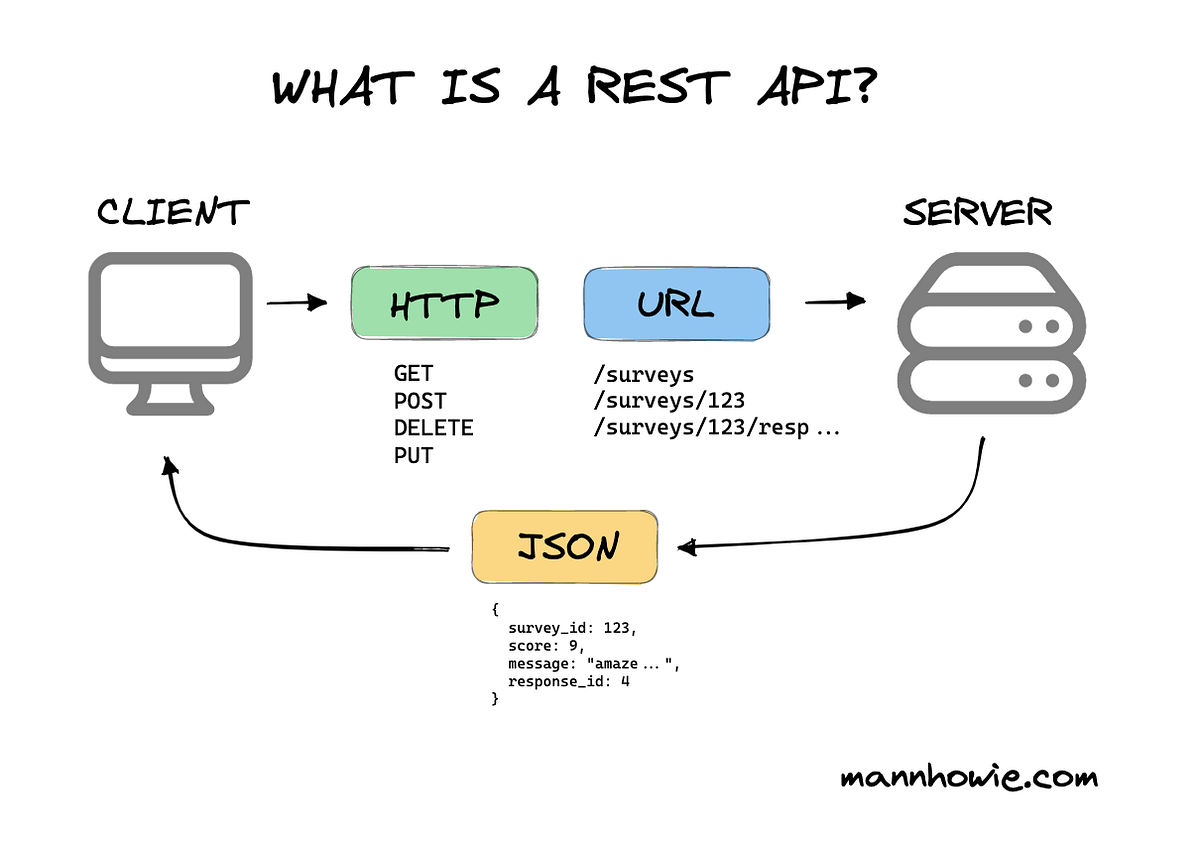
\includegraphics[width=0.80\linewidth]{image/bab2/rest_api.png}
    \caption{Alur RESTful API \citep{howie2023}}
    \label{fig:rest_api}
\end{figure}
Dalam aspek keamanan, RESTful API kini banyak menggunakan OAuth 2.0 dan JWT (JSON Web Token) untuk autentikasi guna mencegah serangan keamanan \textit{man-in-the-middle}. Implementasi fitur \textit{caching} dan \textit{rate limiting} telah meningkatkan efisiensi RESTful API dengan mempercepat respons dan mengurangi beban server. Suatu \textit{request} dapat dianggap dibentuk oleh \textit{endpoint} RESTful API, metode API-yang sebagian besar mencakup operasi CRUD (\textit{GET, PUT, POST, DELETE}) dan parameter. Adapun \textit{status code} mewakili jenis \textit{response} yang diterima dari RESTful API, dengan kode memiliki 3 digit. Digit pertama adalah kategori dengan terbagi menjadi 5 jenis kode, diantaranya yaitu 1xx (proses informasi), 2xx (ok), 3xx (\textit{redirect}), 4xx (\textit{client error}), dan 5xx (\textit{server error}). Digit kedua dan ketiga menunjukkan \textit{status code} dalam rentang digit pertama. IANA (\textit{Internet Assigned Numbers Authority}) mengelola lebih dari 40 kode HTTP resmi \citep{fitri2022}.
\textit{Representational State Transfer Application Programming Interface} (RESTful API) digambarkan sebagai arsitektur layanan web yang memungkinkan komunikasi antara klien dan server menggunakan standar protokol HTTP (\textit{Hypertext Transfer Protocol}). RESTful API dikembangkan sebagai solusi untuk menyediakan antarmuka yang ringan, fleksibel, dan mudah diimplementasikan dalam berbagai platform. Salah satu faktor utama yang menjadikannya standar dalam pengembangan aplikasi web adalah penggunaan format data  JSON, XML dan HTML yang  mudah dibaca dibandingkan format API lainnya \citep{banias2021}.

\section{Flask}
Flask merupakan \textit{lightweight} web \textit{framework} dibangun dari Python, dirancang agar mudah digunakan sejak tahap awal pengembangan. Flask dikategorikan sebagai \textit{micro web framework} karena struktur Flask bersifat minimalis, mudah diintegrasikan dengan \textit{library} Python, serta kompatibel untuk penerapan \textit{machine learning} maupun data \textit{preprocessing} di sisi server \citep{flaskdoc2025}.

Flask memiliki arsitektur modular dan \textit{support} berbagai ekstensi,  memungkinkan pengembangan fitur lanjutan seperti \textit{preprocessing}, autentikasi, hingga (\textit{scheduler}) untuk menjalankan proses tertentu secara berkala. Dalam penelitian ini, Flask dimanfaatkan sebagai komponen \textit{backend}  untuk mengotomasi \textit{preprocessing} data iklim, mulai dari pengambilan data dari sumber BMKG dan NASA POWER, hingga penerapan metode \textit{smoothing}. Hasil pemrosesan selanjutnya disimpan ke dalam \textit{database} MongoDB agar dapat diakses oleh sistem \textit{frontend} Next.js. 
Hal ini sejalan dengan penelitian \cite{singh2019}, bahwa Flask mampu mengelola integrasi data dan proses \textit{database management} secara efisien melalui penggunaan API dan ekstensi, sehingga mendukung otomasi dan skalabilitas sistem \textit{website} \citep{singh2019}.

\section{\textit{Scheduler} Pemrosesan Data}
\textit{Scheduler} merupakan komponen penting dalam menjalankan sistem otomasi proses secara terjadwal tanpa intervensi manual. Menurut \cite{choi2021}, keberhasilan otomasi Python tidak hanya ditentukan oleh kemampuan menulis \textit{script}, tetapi juga oleh mekanisme \textit{runtime execution} sehingga sistem bekerja tanpa kehadiran pengguna. Dengan memanfaatkan layanan cron pada sistem operasi Linux, pengembang dapat menjadwalkan eksekusi \textit{script} Python pada waktu tertentu, sehingga \textit{preprocessing} data menggunakan metode \textit{smoothing} dapat berjalan \citep{choi2021}.

Penelitian \cite{wibowo2025} menjelaskan bahwa penerapan cron job pada infrastruktur \textit{cloud} mampu meningkatkan akurasi, dan konsistensi data secara signifikan. Otomasi \textit{script} dikonfigurasi untuk mentransfer data secara berkala pada interval satu jam menggunakan integrasi Cloud Panel, menghasilkan sistem pemrosesan minim \textit{resources}. Temuan tersebut menunjukkan bahwa \textit{scheduler} berperan penting dalam membangun sistem data \textit{self-updating}. \textit{Scheduler} diintegrasikan dengan \textit{backend} Flask melalui layanan Cronjob untuk mengotomasi \textit{preprocessing}. Setiap kali jadwal eksekusi tercapai, sistem akan menjalankan proses \textit{fetching}, \textit{cleaning}, dan \textit{smoothing} terhadap data iklim dari BMKG, dan NASA POWER secara otomatis. 
\textit{Scheduler} tidak hanya berfungsi sebagai pengatur waktu, tetapi juga memastikan \textit{pipeline} \textit{preprocessing} berjalan konsisten, dan selalu memperbarui data secara berkala \citep{wibowo2025}.

\section{Penelitian Terkait}
Beberapa penelitian memberikan wawasan kepada \saya{} terkait metode penelitian, perancangan sistem dan pemilihan metode \textit{smoothing} yang digunakan. Beberapa penelitian terkait disajikan pada Tabel \ref{tab:penelitian_terkait} berikut:

\renewcommand{\arraystretch}{1.5}
\begin{longtable}{|p{0.05\textwidth}|p{0.27\textwidth}|p{0.33\textwidth}|p{0.25\textwidth}|}
\caption{Penelitian Terkait}
\label{tab:penelitian_terkait}\\
\hline
\textbf{No.} & \textbf{Judul Penelitian} & \textbf{Fokus Utama} & \textbf{Perbedaan} \\
\hline
\endfirsthead

\multicolumn{4}{c}{{Lanjutan Tabel \thetable}}\\
\hline
\textbf{No.} & \textbf{Judul Penelitian} & \textbf{Fokus Utama} & \textbf{Perbedaan} \\
\hline
\endhead

\hline
\multicolumn{4}{r}{Bersambung ke halaman berikutnya}\\
\endfoot

\hline
\endlastfoot

1 &
\textit{Performance of Smoothing Methods for Reconstructing NDVI Time-Series and Estimating Vegetation Phenology from MODIS Data} \citep{cai2017}
&
Membandingkan beberapa metode \textit{smoothing} pada data \textit{time-series} lingkungan, yaitu \textit{Savitzky-Golay}, \textit{LOESS}, \textit{spline smoothing}, \textit{Asymmetric Gaussian}, dan \textit{Double Logistic} untuk memperoleh representasi tren yang lebih akurat pada data NDVI.
&
Berfokus pada data NDVI satelit MODIS untuk analisis fenologi vegetasi, sedangkan penelitian ini menerapkan \textit{smoothing} pada data iklim BMKG dan NASA POWER sebagai dasar penyusunan kalender tanam.
\\ \hline

2 &
\textit{Missing Data Imputation of High-Resolution Temporal Climate Time-Series Data} \citep{afrifa2020}
&
Mengevaluasi berbagai metode imputasi pada data iklim resolusi tinggi, termasuk temperatur, kelembaban, dan kecepatan angin, untuk menentukan metode mana paling efektif dalam mengisi nilai hilang.
&
Penelitian ini berfokus pada perbandingan metode imputasi, sedangkan penelitian yang dilakukan mengintegrasikan imputasi dengan deteksi \textit{outlier}, \textit{smoothing}, dan evaluasi kualitas data dalam satu \textit{pipeline}.
\\ \hline

3 &
\textit{Missing Data Imputation of Climate Time-Series: A Review} \citep{alejo2025}
&
Menyajikan tinjauan komprehensif berbagai metode imputasi data iklim berdasarkan karakteristik variabel, ukuran celah data, dan mekanisme kehilangan data.
&
Bersifat hanya studi literatur. Penelitian ini mengimplementasikan teknik imputasi pada data BMKG dan NASA POWER untuk menghasilkan \textit{dataset} bersih.
\\ \hline

4 &
\textit{Analyzing Error Bounds for Seasonal-Trend Decomposition of Antarctica Temperature Time-Series Involving Missing Data} \citep{kwok2023}
&
Mengkaji penggunaan \textit{Seasonal-Trend decomposition using LOESS} (STL) pada \textit{time-series} suhu yang mengandung nilai hilang serta menganalisis pengaruh kesalahan imputasi terhadap estimasi tren.
&
Berfokus pada analisis teoritis batas galat dekomposisi STL, sedangkan penelitian ini memanfaatkan STL untuk mengevaluasi \textit{trend preservation} setelah proses imputasi dan \textit{smoothing}.
\\ \hline

% 5 &
% \textit{Improving Time Series Data Quality: Identifying Outliers and Handling Missing Values in a Multilocation Gas and Weather Dataset} \citep{alsalehy2025}
% &
% Mengembangkan pendekatan peningkatan kualitas data melalui deteksi outlier dan penanganan nilai hilang pada dataset cuaca dan lingkungan yang berasal dari berbagai lokasi pengamatan.
% &
% Berfokus pada identifikasi outlier dan penanganan data hilang, sedangkan penelitian ini juga mencakup proses \textit{smoothing}, dekomposisi STL, serta evaluasi menggunakan GCV dan \textit{trend preservation}.
% \\ \hline

\end{longtable}

\vspace*{0.8cm} 

\begin{comment}
\end{comment}
